\section{Fundamental of Push Pull Converter}
The push-pull converter is a transformer-based DC-DC converter that efficiently transfers energy between isolated input and output stages. It is widely used in medium-to-high power applications (e.g., telecom systems, renewable energy, and battery chargers) due to its high efficiency, galvanic isolation, and robust performance.
\newpage
\subsection{Basic Operation and Working Principle}
\begin{figure}[h!]
    \centering
    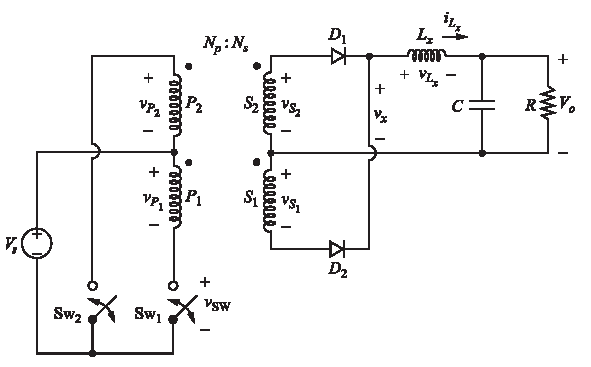
\includegraphics[width=0.8\linewidth]{Pictures/pics/push_pull_circuit.pdf}
    \caption{\textcolor{blue}{\textit{\footnotesize Push-Pull Converter}}}
\end{figure}
\begin{figure}[h!]
    \centering
    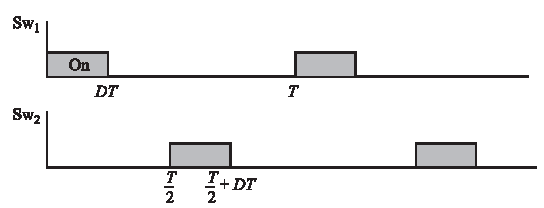
\includegraphics[width=0.8\linewidth]{Pictures/pics/duty_cycle.pdf}
    \caption{\textcolor{blue}{\textit{\footnotesize  Switching sequence}}}
\end{figure}
\subsubsection*{Switch \(S_1\) ON, \(S_2\) OFF}
\begin{itemize}
    \item \textbf{Primary Side:}
    \begin{itemize}
        \item Current flows through \(S_1\) and the \textbf{first half} of the primary winding. 
        \item The transformer core is magnetized in \textbf{one direction}.   
        \item Primary voltage: \(V_{\text{primary}} = V_{\text{in}}\).
    \end{itemize}
    \item \textbf{Secondary Side:}
    \begin{itemize}
        \item The alternating magnetic field induces a voltage in the secondary winding.   
        \item Rectifier diodes convert the AC voltage to DC. 
        \item Output capacitor filters the voltage to power the load.
    \end{itemize}
\end{itemize} 

\subsubsection*{Switch \(S_2\) ON, \(S_1\) OFF}
\begin{itemize}
    \item \textbf{Primary Side}
    \begin{itemize}
        \item Current flows through \(S_2\) and the \textbf{second half} of the primary winding.
        \item Current flows through \(S_2\) and the \textbf{second half} of the primary winding.
        \item The transformer core is magnetized in the \textbf{opposite direction}.
        \item Primary voltage: \(V_{\text{primary}} = V_{\text{in}}\).
    \end{itemize}
    \item \textbf{Secondary Side}
    \begin{itemize}
        \item The reversed magnetic field induces an AC voltage in the secondary winding.
        \item  Rectifier and capacitor continue delivering smooth DC to the load.
    \end{itemize}
\end{itemize}
\subsubsection*{Dead Time: Both Switches OFF}
\begin{itemize}
    \item A brief \textbf{dead time} is inserted between switching transitions to:
    \item Prevent \textbf{shoot-through currents} (both switches conducting simultaneously).
    \item Allow energy from leakage inductance to dissipate via snubber circuits.
    \item Maintain output voltage using the capacitor during transitions.
\end{itemize}    
\subsection{Key Components and Their Roles}
\begin{itemize}
    \item \textbf{Transformer}: Provides galvanic isolation and scales voltage via turns ratio (\(N_p/N_s\))
    \item \textbf{Switches (\(S_1, S_2\))}:  Alternate between ON/OFF states to create AC in the primary (MOSFETs/IGBTs).
    \item \textbf{Rectifier Diodes:} Convert AC voltage on the secondary to pulsating DC.
    \item \textbf{Output Filter (L, C)}: Smooths rectified voltage to stable DC.
    \item \textbf{PWM Controller}: Regulates duty cycle and ensures precise timing.
\end{itemize}